\chapter{Quantum Entanglements, Part 1}

These notes follow Leonard Susskind's seventh lecture on quantum entanglement, curated by LazyingArt LLC. The lecture begins not with entropy but with unfinished business: a stripped-down two-slit experiment, rebuilt in discrete language so that we can see exactly what measurement does to interference. Only after that mechanism is made sharp does Susskind turn to entropy, trace, and density matrices, which he presents as the machinery needed for entanglement entropy in the next lecture.

\section{Finishing the Discrete Two-Slit Setup}

We begin with a very simple model. There is a source at a site labeled \(0\), two openings labeled \(A\) and \(B\), and a screen whose possible arrival sites are denoted by \(|m\rangle\). The rest of the barrier is simply taken to be closed off. For the moment the electron's own spin is ignored; the only degree of freedom we keep is position.

The point of the setup is not geometry but linearity. If a state begins as a superposition, it evolves as the same superposition of the separately evolved parts. In the symmetric case Susskind writes, schematically,
\begin{equation}
|0\rangle \longrightarrow |A\rangle + |B\rangle .
\end{equation}
The board notation suppresses normalization here. If one wished to normalize the state explicitly, one would insert the usual factor \(1/\sqrt{2}\), but the lecture is using shorthand and the relative amplitudes are the important thing.

Each slit state then evolves to a superposition over screen positions:
\begin{align}
|A\rangle &\longrightarrow \sum_m \psi_m |m\rangle , \\
|B\rangle &\longrightarrow \sum_m \phi_m |m\rangle .
\end{align}
The coefficient \(\psi_m\) is the amplitude to arrive at the \(m\)-th screen site starting from \(A\), and \(\phi_m\) is the corresponding amplitude starting from \(B\).

\begin{figure}[h]
\centering

\includegraphics[width=0.72\textwidth]{lecture_07_figure_02.png}
\caption{Lecture board: screen-basis amplitude expansion.}
\end{figure}

The order matters. Susskind first wants us to understand what happens from \(A\) by itself and from \(B\) by itself before we open both holes together. Only then does the genuinely quantum step become unavoidable.

\section{From Path Amplitudes to the Interference Term}

Let us first close one hole at a time. If only \(A\) is open, then at a fixed screen point \(m\) the probability is just
\begin{equation}
P_A(m)=\psi_m^*\psi_m .
\end{equation}
If only \(B\) is open, the corresponding probability is
\begin{equation}
P_B(m)=\phi_m^*\phi_m .
\end{equation}

In classical probability theory one would now be tempted to say that with both holes open the answer is simply \(P_A(m)+P_B(m)\). Susskind pauses exactly here to say: not so in quantum mechanics. We must add amplitudes first.

With both holes open, the state arriving at the screen is
\begin{equation}
|A\rangle + |B\rangle \longrightarrow \sum_n \bigl(\psi_n+\phi_n\bigr)|n\rangle .
\end{equation}
At the particular site \(m\), the amplitude is therefore \(\psi_m+\phi_m\), and the probability is
\begin{align}
P_m &= |\psi_m+\phi_m|^2 \\
&= \psi_m^*\psi_m+\phi_m^*\phi_m+\psi_m^*\phi_m+\phi_m^*\psi_m .
\end{align}
The last two terms are the interference terms. They have no classical analog, and they are the whole reason the experiment is interesting.

At the symmetry point on the screen we expect, by symmetry,
\begin{equation}
\psi_m=\phi_m ,
\end{equation}
so the probability is enhanced. In Susskind's board shorthand one gets four times the single-route contribution. On the other hand, if by shifting the observation point or the beam preparation we arrange
\begin{equation}
\psi_m=-\phi_m ,
\end{equation}
then
\begin{equation}
P_m=0 .
\end{equation}
The electron can reach \(m\) through either slit separately, but with both slits open it does not arrive there at all. This is the peculiar algebraic fact that drives the rest of the lecture.

\begin{figure}[h]
\centering

\includegraphics[width=0.74\textwidth]{lecture_07_figure_03.png}
\caption{Lecture board: interference probability and cross terms.}
\end{figure}

\section{Which-Path Recording as Entanglement with a Spin}

Now comes the real question. What happens if some device records which slit the electron used?

Susskind introduces the simplest possible apparatus: an auxiliary spin with two states, \(u\) and \(d\). This is not, at this stage, the electron's own spin. It is an external degree of freedom that can serve as a record. The initial state is the electron at the source with the detector untriggered:
\begin{equation}
|0,d\rangle .
\end{equation}
The rule of the model is that passage through slit \(A\) flips the apparatus spin from down to up, whereas passage through slit \(B\) leaves it down. Thus the schematic update is
\begin{equation}
|0,d\rangle \longrightarrow |A,u\rangle + |B,d\rangle .
\end{equation}
From that point onward the electron continues toward the screen just as before, while the detector state simply tags the route:
\begin{align}
|A,u\rangle &\longrightarrow \sum_n \psi_n |n,u\rangle , \\
|B,d\rangle &\longrightarrow \sum_n \phi_n |n,d\rangle .
\end{align}
So the final state is
\begin{equation}
|\Psi_{\mathrm{final}}\rangle
=
\sum_n \bigl(\psi_n |n,u\rangle + \phi_n |n,d\rangle\bigr) .
\end{equation}

This is already the essential idea. The electron is no longer described by a lone superposition over routes. The route alternatives have become correlated with orthogonal detector states.

\subsection{Question \& Answer}

\paragraph{Question.} Did the wave packet collapse, or did the electron become entangled with the detector?

\paragraph{Answer.} Susskind's answer is deliberately sharp. If we ignore the apparatus and describe only the electron, then one may use the language of collapse: the interference terms are gone, and one says the electron has been forced into one route or the other. But if we keep the apparatus inside the quantum description, then that language is too crude. The composite system has not yet become one branch or the other; it has become an entangled state,
\[
|A,u\rangle + |B,d\rangle .
\]
In that fuller description the correct statement is not that collapse has occurred, but that entanglement has been established. Collapse is a later shorthand for forgetting part of the system.

This is why the lecture keeps insisting on the apparatus. Once entanglement enters the story, loose talk about measurement must be replaced by a concrete correlation between system and detector.

\section{Projector onto a Screen Position and Loss of Cross Terms}

Susskind then returns to formalism and does the calculation carefully. We want the probability that the electron is found at the screen point \(m\). In the enlarged Hilbert space, there are two orthogonal states with that property:
\[
|m,u\rangle
\qquad \text{and} \qquad
|m,d\rangle .
\]
Therefore the projector onto ``electron at \(m\)'' is
\begin{equation}
\Pi_m = |m,u\rangle\langle m,u| + |m,d\rangle\langle m,d| .
\end{equation}

\begin{figure}[h]
\centering

\includegraphics[width=0.68\textwidth]{lecture_07_figure_04.png}
\caption{Lecture board: projector onto a fixed screen position.}
\end{figure}

The probability is the expectation value of this projector in the final state:
\begin{equation}
P_m = \langle \Psi_{\mathrm{final}}|\Pi_m|\Psi_{\mathrm{final}}\rangle .
\end{equation}
Substituting the final state gives
\begin{align}
P_m
&=
\sum_{n,n'}
\bigl(\psi_n^*\langle n,u|+\phi_n^*\langle n,d|\bigr)
\Pi_m
\bigl(\psi_{n'}|n',u\rangle+\phi_{n'}|n',d\rangle\bigr) .
\end{align}
Now the logic of the projector does all the work. The bra \(\langle n,u|\) can contribute only against \(|m,u\rangle\), and only when \(n=m\). Likewise \(\langle n,d|\) contributes only against \(|m,d\rangle\), again only when \(n=m\). The mixed terms try to pair \(u\) with \(d\), and these vanish because
\begin{equation}
\langle u|d\rangle = 0 .
\end{equation}
Hence
\begin{equation}
P_m = |\psi_m|^2 + |\phi_m|^2 .
\end{equation}

This is the formal centerpiece of the lecture. The cross terms do not disappear by decree; they disappear because the would-be interfering branches now end in orthogonal detector states. The electron amplitude from \(A\) multiplies one ket vector and the amplitude from \(B\) multiplies another. Since the record states are distinguishable, the amplitudes no longer combine into a single probability amplitude at fixed \(m\).

\section{What Counts as a Measurement?}

After the clean spin model is in place, the lecture widens into a long clarification of what should count as a measurement. The answer is deliberately broad: a measurement occurs whenever a record is left in the world that can, in principle, distinguish the alternatives. The record need not be read by a human observer. It is enough that it exists.

\subsection{Question \& Answer}

\paragraph{Question.} What counts as a measurement?

\paragraph{Answer.} Anything that leaves a mark from which one can infer, fully or even partially, which route the electron took. If the mark is perfectly distinguishing, the interference is destroyed. If it distinguishes only imperfectly, the interference is only partially destroyed.

The lecture first tests the symmetric case. Suppose the apparatus spin is placed so symmetrically that it is kicked in exactly the same way whether the electron passes through \(A\) or through \(B\). Then the two branches produce the same record state, so the post-slit state is effectively
\begin{equation}
|A,u\rangle + |B,u\rangle .
\end{equation}
Now the spin tells us nothing about which hole was used, and the interference pattern remains.

\begin{figure}[h]
\centering

\includegraphics[width=0.72\textwidth]{lecture_07_figure_05.png}
\caption{Lecture board: symmetric placement of the spin detector.}
\end{figure}

\begin{figure}[h]
\centering
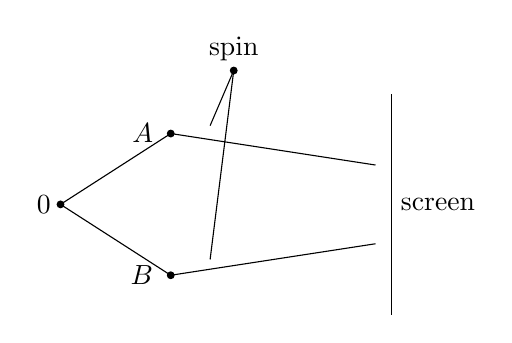
\begin{tikzpicture}[scale=1.0]
\fill (-2,0) circle (0.05);
\node[left] at (-2,0) {$0$};

\fill (-0.6,0.9) circle (0.05);
\node[left] at (-0.7,0.9) {$A$};

\fill (-0.6,-0.9) circle (0.05);
\node[left] at (-0.7,-0.9) {$B$};

\draw (-2,0) -- (-0.6,0.9);
\draw (-2,0) -- (-0.6,-0.9);

\draw (-0.6,0.9) -- (2.0,0.5);
\draw (-0.6,-0.9) -- (2.0,-0.5);

\draw (2.2,-1.4) -- (2.2,1.4);
\node[right] at (2.2,0) {screen};

\fill (0.2,1.7) circle (0.05);
\node[above] at (0.2,1.7) {$\mathrm{spin}$};

\draw (0.2,1.7) -- (-0.1,1.0);
\draw (0.2,1.7) -- (-0.1,-0.7);
\end{tikzpicture}
\caption{Clean schematic of the symmetric detector placement.}
\end{figure}

The recoil example makes the same point more subtly. If the slit plate recoils differently depending on the route, then the plate itself can serve as a record. But if the kick is small compared with the intrinsic spread of the plate's momentum wave function, the two recoil states overlap strongly and are not orthogonal. In that case one gets only partial loss of interference. The lecture does not turn this into a long formal detour, but the organizing formula is simple:
\begin{equation}
P_m
=
|\psi_m|^2+|\phi_m|^2
+\psi_m^*\phi_m\langle E_A|E_B\rangle
+\phi_m^*\psi_m\langle E_B|E_A\rangle ,
\end{equation}
where \(|E_A\rangle\) and \(|E_B\rangle\) are the record states of the apparatus or environment. Orthogonality, \(\langle E_A|E_B\rangle=0\), means complete which-path information and no interference. Large overlap means that interference survives.

The same reasoning then covers partial spin kicks, emitted photons, and bubble-chamber tracks. A slow electron may emit a photon only occasionally, so the radiation field records route information only imperfectly and the fringes are merely blurred. A bubble chamber or any track-forming device leaves a much more robust record, and interference is gone.

Two points are emphasized repeatedly. First, one does not have to look at the apparatus. The record itself is enough. Second, the lecture treats the order of observation as secondary. If there exists a later measurement that can reveal which path was taken, then the branches were already correlated with distinct records, and the interference is absent for that reason.

\section{Measurement Chains, Schr\"odinger's Cat, and the Movable Cut}

From here Susskind enlarges the same mathematics rather than changing it. Schr\"odinger's cat is not a new subject; it is the same subject with a larger apparatus.

Suppose the cat is tied to a gun that may or may not fire. The composite system evolves to a state of the form
\begin{equation}
|\Psi_{\mathrm{cat}}\rangle
=
\alpha\,|{\rm live},{\rm unfired}\rangle
+
\beta\,|{\rm dead},{\rm fired}\rangle .
\end{equation}
The important point is what this is not. It is not a lone cat state
\[
\alpha\,|{\rm live}\rangle+\beta\,|{\rm dead}\rangle .
\]
The cat is entangled with the gun, and the gun has already left a mark. Therefore there are no interference terms between ``live'' and ``dead'' when we ask ordinary observational questions about the cat. Exactly as in the slit experiment, the alternatives are attached to orthogonal records.

The same logic continues when Schr\"odinger looks in the box, and then when Wigner asks Schr\"odinger what he saw. Each new observer can be included as one more system that becomes correlated with the earlier systems. The cut between ``system'' and ``observer'' is therefore movable. One may stop at the electron and say its wave function collapsed. One may stop at electron plus detector and say that combined state collapsed. Or one may include the observer as well. The lecture's claim is not that this ambiguity disappears, but that the predictions remain consistent whichever cut one uses.

This is also why Susskind insists that the final detection screen is itself another measurement device. A photographic plate blackens; a scintillation screen emits light; a row of spins can flip at the point of impact. In each case the arrival position becomes entangled with some macroscopic record. At that stage we speak of probabilities because quantum mechanics tells us to compute the expectation value of the corresponding projector. Nothing mystical is added at the screen; only one more round of entanglement.

The broader contrast with classical physics is also made explicit. In classical mechanics one imagines that a sufficiently gentle measurement need not appreciably disturb the system. In quantum mechanics, the measurement that determines among incompatible alternatives must establish entanglement with an apparatus, and that is a genuine change of state. Measurement is not external bookkeeping. It is a physical interaction that changes whether interference survives.

\section{Entropy, Trace, Density Matrix, and the Next Step}

At this point the lecture pivots hard. Susskind says, in effect, that what he really wanted was a quantitative measure of entanglement, but before he can define it he needs some machinery.

He begins with the simplest contrast. Two spins both up form an unentangled product state. Looking at one tells us nothing new about the other. Entangled states are different, and the standard measure he wants to reach is entanglement entropy. But first we go back to classical entropy.

Suppose a classical system can occupy a finite collection of states, and all we know is that it lies in one of \(n\) equally likely possibilities. Then the entropy is defined to be
\begin{equation}
S=\log n .
\end{equation}
More generally, if the probability distribution is \(p_i\), then
\begin{equation}
S=-\sum_i p_i\log p_i .
\end{equation}
The minus sign is there because probabilities are less than one, so their logarithms are negative.

The lecture checks that the general formula reproduces the equal-probability case. If
\begin{equation}
p_i=\frac{1}{n}
\qquad \text{for } i\in \mathcal N,
\qquad
p_i=0
\qquad \text{for } i\notin \mathcal N ,
\end{equation}
with \(|\mathcal N|=n\), then
\begin{align}
S
&=
-\sum_i p_i\log p_i \\
&=
-n\left(\frac{1}{n}\right)\log\left(\frac{1}{n}\right) \\
&=
\log n .
\end{align}
So the Shannon formula really is the correct generalization of the simpler \(\log n\) definition.

Before going on to density matrices, Susskind introduces the trace.

\begin{definition}
For an operator \(M\) and any complete orthonormal basis \(\{|i\rangle\}\), the trace is
\begin{equation}
\operatorname{Tr} M = \sum_i \langle i|M|i\rangle .
\end{equation}
\end{definition}

The crucial point is that this does not depend on the basis. In a basis where \(M\) is diagonal, the diagonal entries are its eigenvalues, and therefore
\begin{equation}
\operatorname{Tr} M = \sum_i \lambda_i .
\end{equation}
This basis-independence is what makes the trace the right quantum replacement for summing over classical alternatives.

The lecture then turns to the case in which someone prepares a system in one basis state \(|i\rangle\), but does not tell us which one. We are told only the preparation probabilities \(\rho_i\). This is not a coherent superposition with definite phases. It is ignorance about preparation. The appropriate object is a density matrix.

\begin{figure}[h]
\centering

\includegraphics[width=0.70\textwidth]{lecture_07_figure_06.png}
\caption{Lecture board: schematic transition to a density-matrix description.}
\end{figure}

\begin{figure}[h]
\centering
\begin{tikzpicture}[scale=1.0]
\node at (-2.3,0) {$|\psi\rangle$};
\draw[->] (-1.6,0) -- (-0.4,0);

\draw (1.1,0) circle (1.2);
\fill (0.5,0.5) circle (0.05);
\fill (1.4,0.6) circle (0.05);
\fill (0.7,-0.2) circle (0.05);
\fill (1.6,-0.4) circle (0.05);
\fill (1.1,0.1) circle (0.05);

\node at (1.1,-1.6) {$\rho$};
\end{tikzpicture}
\caption{Clean schematic of the move from a state-vector description to a statistical description.}
\end{figure}

In the basis of preparation states, the density matrix is diagonal:
\begin{equation}
\rho=
\mathrm{diag}(\rho_1,\rho_2,\rho_3,\ldots) .
\end{equation}
Because the probabilities sum to one,
\begin{equation}
\operatorname{Tr}\rho=1 .
\end{equation}

Now let \(F\) be an observable, represented by a Hermitian operator. The lecture's central formula is
\begin{equation}
\langle F\rangle = \operatorname{Tr}(F\rho) .
\end{equation}
This is the quantum analog of the classical average \(\sum_i p_i f_i\).

To see why, insert a resolution of the identity between \(F\) and \(\rho\):
\begin{equation}
\sum_j |j\rangle\langle j| = I .
\end{equation}
Then
\begin{align}
\langle F\rangle
&=
\operatorname{Tr}(F\rho) \\
&=
\sum_i \langle i|F\rho|i\rangle \\
&=
\sum_{i,j}\langle i|F|j\rangle\langle j|\rho|i\rangle .
\end{align}
If we choose the basis in which \(\rho\) is diagonal, then \(\langle j|\rho|i\rangle=0\) unless \(i=j\). Hence
\begin{align}
\langle F\rangle
&=
\sum_i \langle i|F|i\rangle \rho_i \\
&=
\sum_i F_{ii}\rho_i .
\end{align}
This is exactly what it should be: the expectation value of \(F\) in each possible preparation state, weighted by the probability that the system was prepared in that state.

The lecture also notes the cyclic property
\begin{equation}
\operatorname{Tr}(AB)=\operatorname{Tr}(BA) ,
\end{equation}
which holds even when \(A\) and \(B\) do not commute. This is why it does not matter whether we write \(\operatorname{Tr}(F\rho)\) or \(\operatorname{Tr}(\rho F)\).

Finally, Susskind gives the quantum entropy associated with a density matrix:
\begin{equation}
S=-\operatorname{Tr}(\rho\log\rho) .
\end{equation}
If \(\rho\) is diagonal, then \(\log\rho\) is simply the diagonal matrix of logarithms of the eigenvalues:
\begin{equation}
\log\rho
=
\mathrm{diag}(\log\rho_1,\log\rho_2,\log\rho_3,\ldots) .
\end{equation}
So in that case
\begin{equation}
S=-\sum_i \rho_i \log\rho_i .
\end{equation}
If only one eigenvalue is \(1\) and all the others are \(0\), then the entropy is zero. That is the pure-state case. If \(\rho\) is proportional to the identity, so that all states are equally likely, then the entropy is the logarithm of the dimension of the state space:
\begin{equation}
\rho \propto I
\qquad \Longrightarrow \qquad
S=\log(\dim \mathcal H) .
\end{equation}

This is where the lecture stops. The key promise is reserved for next time: if a composite system \(AB\) is entangled, then the density matrix that describes \(A\) alone will have nonzero entropy; if \(A\) and \(B\) are not entangled, it will not. The whole entropy discussion in this lecture is therefore preparatory. It supplies the language in which entanglement entropy can later be defined.

\section{Summary}

The lecture has two tightly connected movements. First, it rebuilds the two-slit experiment in discrete form and shows that interference disappears when the alternative routes become entangled with orthogonal record states. Measurement is therefore not introduced as a mysterious extra rule but as the establishment of system-apparatus entanglement. Second, having made that mechanism concrete, the lecture changes gears and develops the tools needed to measure entanglement quantitatively: classical entropy, the trace, density matrices, expectation values of the form \(\operatorname{Tr}(F\rho)\), and the entropy \(S=-\operatorname{Tr}(\rho\log\rho)\). The actual definition of entanglement entropy is postponed, but by the end of the lecture all the necessary ingredients are on the board.